\documentclass{article}



\usepackage{arxiv}

\usepackage[utf8]{inputenc} % allow utf-8 input
\usepackage[T1]{fontenc}    % use 8-bit T1 fonts
\usepackage{hyperref}       % hyperlinks
\usepackage{url}            % simple URL typesetting
\usepackage{booktabs}       % professional-quality tables
\usepackage{amsfonts}       % blackboard math symbols
\usepackage{nicefrac}       % compact symbols for 1/2, etc.
\usepackage{microtype}      % microtypography
\usepackage{lipsum}		% Can be removed after putting your text content
\usepackage{graphicx}
\usepackage{natbib}
\usepackage{doi}
\usepackage{amsmath}
\usepackage{amsthm}
\usepackage{tikz}
\usepackage{pgfplots}
\usepackage{todonotes}
\usepackage{caption}
\usepackage{subcaption}
\usepackage{float}
\usetikzlibrary{patterns}
\usepgfplotslibrary{fillbetween}
\pgfplotsset{compat=1.17}
\newtheorem{theorem}{Theorem}
\newtheorem{proposition}{Proposition}


\title{Multidimensional Extension of Buffon's Needle Problem}

%\date{September 9, 1985}	% Here you can change the date presented in the paper title
%\date{} 					% Or removing it

\author{ Alexander~Choi\\
	alexander.e.choi@gmail.com
}

% Uncomment to remove the date
%\date{}

% Uncomment to override  the `A preprint' in the header
%\renewcommand{\headeright}{Technical Report}
%\renewcommand{\undertitle}{Technical Report}
\renewcommand{\shorttitle}{Multidimensional Buffon's Needle}

%%% Add PDF metadata to help others organize their library
%%% Once the PDF is generated, you can check the metadata with
%%% $ pdfinfo template.pdf
\hypersetup{
pdftitle={Multidimensional Extension of Buffon's Needle Problem},
pdfsubject={q-bio.NC, q-bio.QM},
pdfauthor={Alexander E.~Choi},
pdfkeywords={Buffon's needle problem, Geometric probability},
}

\begin{document}
\maketitle

\begin{abstract}
	Consider a line segment randomly placed on a two-dimensional plane ruled with a set of regularly spaced parallel lines. The classical Buffon's needle problem
    asks what the probability is that the line segment intersects at least 1 of these lines. This paper extends this problem by considering a line segment randomly
    placed in $\mathbb{R}^D$ and its probability of intersection with a set of regularly spaced parallel hyperplanes. 
\end{abstract}


% keywords can be removed
\keywords{Buffon's needle problem \and Geometric Probability}

\section{Introduction}
Buffon's needle problem was originally posed in the 18th century with the following premise. Given a line segment, or "needle", of length $r$ randomly dropped on a two-dimensional plane
ruled with a set of parallel lines regularly spaced $s$ units apart, what is the probability that the needle crosses at least 1 of the lines? The solution, it turns out, is
$\frac{2r}{s\pi}$ when $r<s$. Variations and extensions of this problem have been investigated as well, including
\begin{itemize}
	\item Laplace's Extension - Investigating when the plane is gridded with 2 orthogonal sets of parallel lines with spacings $s_1$ and $s_2$.
	\item Buffon's Noodle - Instead of being rigidly straight, the needle is permitted to bend (a "noodle").
	\item Pivot Needle - The needle is constructed of two line segments that hinge together. Each crossing is considered.
\end{itemize}

In this paper, we investigate a particular extension that allows the needle to be dropped into a space with dimension greater than 2. In these higher dimensions, we will rule the space
with parallel hyperplanes rather than lines. Additionally, we will look at gridding the space with orthogonal sets of hyperplanes, thereby extending Laplace's extension into higher dimensions.

Given $D\in\mathbb{N}_{>0}$ and $N\in[1,2,\dots,D]$, consider a grid on $\mathbb{R}^D$ formed by $N$ orthogonal sets of regularly spaced hyperplanes. Each set of hyperplanes
has a potentially unique spacing of $S_i$. For example, if $D=2, N=1, S_1=2$, the grid would match the original Buffon Needle problem and would have only a single set of parallel lines 2 units apart as seen in \ref{fig:buffon example}.
If $D=2, N=2, S=[2, 1]$, the grid would have 2 sets of parallel lines that are orthogonal to each other, matching the problem in Laplace's extension as seen in \ref{fig:laplace example}. One set of lines would have a spacing of 2 units and 
the other would have a spacing of 1 unit.

A line segment of length $r\in\mathbb{R}^+$ is randomly located in the space such that one of its end points, $P_0$, is uniformly distributed
across the entire domain. The line segment's orientation is independently distributed such that when considering $P_0$ as the center of a $(D-1)$-sphere of radius $r$, the other point, $P_1$,
is uniformly distributed on the surface of that hypersphere. This line segment may intersect with $C\in\mathbb{N}$ unique hyperplanes. This paper studies the probability that the line segment
intersects with at least $c$ hyperplanes, $P(C\ge c|r, D, N, S)$. From there, solutions for crossing at most $c$ hyperplanes and exactly $c$ hyperplanes can
be derived.
\begin{figure}[H]
	\centering
	\begin{subfigure}{0.45\textwidth}
		\centering
		\begin{tikzpicture}
			% Buffon Needle lines
			\foreach \x in {0,1,2,...,5} {
			\draw (\x,0) -- (\x,3);
			}
			% Needle
			\draw[thick] (2.2,1.5) -- (3.2,2) node[midway, above] {$r$};
			\draw[<->] (2,1) -- (3,1) node[midway, below] {$S_1$};
		\end{tikzpicture}
		\caption{$D=2, N=1, S_1=2$, the parameter set matching Buffon's Needle Problem. In this case the number of crossings, $C$, is 1.}
		\label{fig:buffon example}
	\end{subfigure}
	\hspace{1cm}
	\begin{subfigure}{0.45\textwidth}
		\centering
		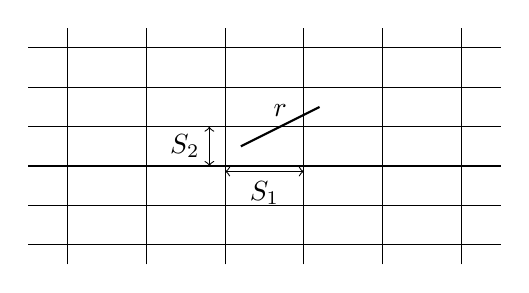
\begin{tikzpicture}
			% Laplace Extension lines
			\foreach \x in {0,1,2,...,5} {
			\draw (\x,0) -- (\x,3);
			}
			\foreach \y in {0.25,0.75,...,2.75} {
			\draw (-0.5,\y) -- (5.5,\y);
			}
			% Needle
			\draw[thick] (2.2,1.5) -- (3.2,2) node[midway, above] {$r$};
			\draw[<->] (2,1.18) -- (3,1.18) node[midway, below] {$S_1$};
			\draw[<->] (1.8,1.25) -- (1.8,1.75) node[left, midway] {$S_2$};
		\end{tikzpicture}
		\caption{$D=2, N=2, S=[2,1]$, the parameter set matching Laplace's Extension. In this case the number of crossings, $C$, is 2.}
		\label{fig:laplace example}
	\end{subfigure}
	\caption{Examples of different parameter sets}
\end{figure}

We will define the coordinates of line segment using $\vec{x}\in\mathbb{R}^D$ for the location of $P_0$ and spherical coordinates for the location of $P_1$ with respect to $P_0$.

\begin{align*}
    y_1 &= r\cos{\phi_1}\\
    y_2 &= r\sin{\phi_1}\cos{\phi_2}\\
    \vdots\\
    y_{D-1} &= r\sin{\phi_1}\hdots\sin{\phi_{D-2}}\cos{\phi_{D-1}}\\
    y_{D} &= r\sin{\phi_1}\hdots\sin{\phi_{D-2}}\sin{\phi_{D-1}}\\
    P_1 &= \vec{x} + \vec{y}\\
	\phi_j &\in \begin{cases}[0, \pi] & j<D-1 \\ [0, 2\pi] & j=D-1\end{cases}
\end{align*}

The selection of basis vectors provide simplifications to the problem. Translational symmetry of the selection
of $P_0$ allows the origin to be freely moved without loss of generaliztion. By placing the origin of the coordinate
system on a vertex of the grid cell containing $P_0$ and constraining the basis vectors to be collinear with the
edges of that grid cell, the domain of $x_i$ is constrained to $[0, S_i]$. The particular vertex can be chosen
to ensure that the needle is oriented in the direction of a particular orthant. For convenience, we will choose
the orthant such that $\phi_i \in [0, \pi/2].$
% Translational symmetry of the grid of hyperplanes allows us to consider the domain of $P_0$ to be $x_i\in[0,S_i]$ as the gridcell containing $P_0$ can be redefined as 
% the grid cell at the origin. Reflectional symmetry of the grid also allows us to consider the domain of $\vec{y}$ to be a single orthant of the hypersphere as the basis
% vectors $\hat{e_i}$ can be reflected to ensure that the needle's orientation is directed in a certain orthant. For convenience, we will pick the orthant where
% $\phi_i \in [0, \pi/2]$.

The rest of the paper is organized as follows. A derivation of the joint probability density function for $P_0$ and $P_1$ will be provided in \S \ref{s:needle pdf}. The derivation and validation
of the crossing probabilities for $N=1$ will be given in \S \ref{s:n=1}. The derivation and validation of the crossing probabilities for all $N$ and $r<\min(S)$ will be given in \S 4. Numeric
simulation of the crossing probabilities will be compared to modeled probabilities in \S 5, along with analysis of the limits
and extrema of the probabilities.

\section{Joint Probability Density of the Line Segment} \label{s:needle pdf}
Each coordinate for $P_0$ can be defined as a uniformly distributed random variable $X_i\sim{\rm Uniform}(0,S_i)$. Due to independence, the joint PDF for $P_0$ is the product
$\prod_{i=1}^D \frac{1}{S_i}$. By the definition of the problem, the coordinates $\vec{x}$ do not influence the orientation of the line segment defined by $\vec{\phi}$. 
The probability density function for the uniform distribution of points on an orthant of the hypersphere can be determined by calculating the area element in terms of spherical coordinates.

\todo{This doesn't seem like it needs to be a prop as it's only really used once. Maybe the prop should be the PDF of the whole segment}
\begin{proposition}
In spherical coordinates, the probability density function for a uniform distribution on an orthant of a hypersphere is $\frac{2^D}{A_{D-1}}\prod_{j=1}^{D-1}r\sin^{D-1-j}\phi_j$ where
$A_{D-1}$ is the surface area of a $(D-1)$-sphere.
\end{proposition}
\begin{proof}
	The area element of an $(D-1)$-sphere of radius $r$ can be expressed as 
	\begin{equation} \label{eq:1}
	d\Omega = \left(\prod_{j=1}^{D-1}r\sin^{D-1-j}\phi_j\right)d\phi_1 \hdots d\phi_{D-1}
	\end{equation}
	The probability that a point lies in this differential element can be expressed as follows.
	\begin{equation} \label{eq:2}
	f_{\Omega}(\Omega)d\Omega = f_{\vec{\phi}}(\phi_1, \hdots, \phi_{D-1})d\phi_1 \hdots d\phi_{D-1}
	\end{equation}
	The points are uniformly distributed over the surface of an orthant of the hypersphere implying that $f_{\Omega}(\Omega) = \frac{2^D}{A_{D-1}}$. Substituting this and
	\ref{eq:1} into \ref{eq:2} yields
	\begin{equation}
	\frac{2^D}{A_{D-1}}\prod_{j=1}^{D-1}r\sin^{D-1-j}\phi_j = f_{\vec{\phi}}(\phi_1, \hdots, \phi_{D-1})
	\end{equation}
\end{proof}

Then by independence, the joint probability density function for the entire line segment can be expressed as 
\begin{equation} 
	f_{\vec{X},\vec{\phi}}(x_1, \hdots, x_D, \phi_1, \hdots, \phi_{D-1}) = \frac{2^D}{A_{D-1}}\left(\prod_{i=1}^D\frac{1}{S_i}\right)\left(\prod_{j=1}^{D-1}r\sin^{D-1-j}\phi_j\right)
\end{equation} 

The expression for the surface area of a $D-1$ dimensional hypersphere, $A_{D-1}=\frac{2\pi^{D/2}r^{D-1}}{\Gamma(D/2)}$,
can be substituted in and simplified.

\begin{equation}\label{eq:general pdf}
	f_{\vec{X},\vec{\phi}}(\vec{x}, \vec{\phi}) = \frac{2^{D-1}\Gamma(\frac{D}{2})}{\pi^{D/2}\prod_{i=1}^DS_i} \left(\prod_{j=1}^{D-1}\sin^{D-1-j}\phi_j\right)
\end{equation}

\section{Probability of Crossing with a Single set of Hyperplanes ($N=1$)} \label{s:n=1}
In general, the probability of meeting some number of crossings given any set of parameters can be described as follows.

\begin{align} 
	P(C\ge c|r, D, N, S)&=\idotsint_V f_{\vec{X}\vec\phi}(\phi_1,\hdots,\phi_{D-1})dx_1 \hdots dx_D d\phi_1 \hdots d\phi_{D-1} \label{eq:raw integral}\\
	&= \frac{2^{D-1}\Gamma(\frac{D}{2})}{\pi^{D/2}\prod_{i=1}^DS_i} \idotsint_V \prod_{j=1}^{D-1}\sin^{D-1-j}\phi_j dx_1\hdots dx_D d\phi_1 \hdots d\phi_{D-1} \label{eq:volume integral}
\end{align}

Where $V$ is the hypervolume in which the condition $C\ge c$ is true. The necessary conditions for achieving some number of intersections
will be called \emph{crossing conditions}. The definition of these crossing conditions and the solution to the above equation will be
explored for a variety of parameters.
We start with a simplified set of parameters where there is only a single set of parallel hyperplanes and the needle intersects a
hyperplane at least $c$ times. That is, the probability $P(C\ge c | r, D, N=1, S) \forall c, r, D, S$. For brevity, we will refer to this
as $P_{N=1}(c)$.

Due to rotational symmetry of the line segment, it does not matter in which direction the hyperplanes extend. Without loss of
generality we assume the planes are in the direction of $x_1$.

Because $P_0$ is constrained to be within the gridcell at the origin and because the orientation of the needle is constrained to a single
orthant which points in the positive direction of $x_1$, we know that a crossing occurs whenever the following condition is met.
\begin{equation}
	x_1 + r\cos{\phi_1} > S_1c
\end{equation}

From this crossing condition, we define the bounds of the relevant hypervolume. Note that the constraints above only apply to $x_1$ and
$\phi_1$. As such, the hypervolume spans the entire domain of every other variable. Importantly, because the integrand of \ref{eq:raw integral}
describes a PDF, the conditions for Fubini's theorem hold. Therefore the order of integration can be freely switched so long as any variable
limits of integration are accounted for. All integrals with respect to the translational dimensions $x_2, \hdots, x_D$ can be simplified
for all $i>2$. Taking $f(\vec\phi)$ as the integrand
\begin{equation}
	\int_0^{S_i}f(\vec\phi)dx_i = S_if(\vec\phi) \label{eq:irrelevant translational}
\end{equation}

Similarly, all of the integrals with respect to $\phi_2, \hdots, \phi_{D-1}$ can be simplified as well using the following identity.
\begin{equation}
	\int_0^{\pi/2}\sin^{D-1-j}\phi_jd\phi_j = \frac{B(\frac{D-j}{2}, \frac{1}{2})}{2}\label{eq:irrelevant rotational}
\end{equation}

Where $B$ is the beta function. Substituting \ref{eq:irrelevant translational} and \ref{eq:irrelevant rotational} into 
\ref{eq:volume integral} results in
\begin{equation} \label{eq:preproduct simplification}
	P_{N=1}(c) = \frac{2^{D-1}\Gamma(\frac{D}{2})}{\pi^{D/2}S_1} \prod_{k=2}^{D-1}\frac{B(\frac{D-k}{2}, \frac{1}{2})}{2} \iint_{\phi_1,x_1}\sin^{D-2}\phi_1 dx_1 d\phi_1
\end{equation}

The product of beta functions can be simplified by expanding into gamma functions as follows.
\begin{align}
	\prod_{k=2}^{D-1}\frac{B(\frac{D-k}{2}, \frac{1}{2})}{2} &= \frac{1}{2^{D-2}} \frac{\Gamma(\frac{D-2}{2})\Gamma(\frac{1}{2})}{\Gamma(\frac{D-1}{2})} \frac{\Gamma(\frac{D-3}{2})\Gamma(\frac{1}{2})}{\Gamma(\frac{D-2}{2})} \hdots \frac{\Gamma(\frac{1}{2})\Gamma(\frac{1}{2})}{\Gamma(\frac{2}{2})} \\
	&= \frac{1}{2^{D-2}} \frac{\Gamma(\frac{1}{2})\Gamma(\frac{1}{2})^{D-2}}{\Gamma(\frac{D-1}{2})} = \frac{\pi^{(D-1)/2}}{2^{D-2}\Gamma(\frac{D-1}{2})} \label{eq:beta prod}
\end{align}

Substituting \ref{eq:beta prod} into \ref{eq:preproduct simplification} yields
\begin{equation}
	P_{N=1}(c) = \frac{2}{S_1B(\frac{D-1}{2}, \frac{1}{2})} \iint_{\phi_1,x_1}\sin^{D-2}\phi_1 dx_1 d\phi_1 \label{eq:n=1 int}
\end{equation}

For the remaining integrals, the limits of integration are defined by the domain in which the crossing conditions are satisfied. This
can be derived by combining the domains for the variables and the domain for the crossing condition. Recall the following
\begin{gather*}
	0 < x_1 < S_1 \\
	0 < \phi_1 < \frac{\pi}{2} \\
	x_1 + r\cos\phi_1 > S_1c
\end{gather*}

Combining these inequalities results in the following domain where the crossing conditions are satisfied.
\begin{gather}
	\max(0, S_1c-r\cos\phi_1) < x_1 < S_1 \label{eq:x cross cond} \\
	0 < \phi_1 < \min(\frac{\pi}{2}, \arccos\frac{S_1c-x_1}{r}) \label{eq:phi cross cond} \\
	r > \frac{S_1c - x_1}{\cos{\phi_1}} \label{eq:r cross cond}
\end{gather}

The min function in \ref{eq:phi cross cond} can be simplified to $\arccos\frac{S_1c-x_1}{r}$ as the conditions for the alternative are
only possible in the trivial case where $c=0$ as shown below.
\begin{align}
	m_{\phi_1}(x_1) = \min(\frac{\pi}{2}, \arccos\frac{S_1c-x_1}{r}) &= \begin{cases}
		\frac{\pi}{2} & x_1>S_1c \\
		\arccos\frac{S_1c-x_1}{r} & \text{otherwise}
	\end{cases} \\
	&= \arccos\frac{S_1c-x_1}{r} 
\end{align}

The final inequality, \ref{eq:r cross cond}, provides a lower bound for the parameter $r$. The minimum of $\frac{S_1c - x_1}{\cos{\phi_1}}$
occurs at $x_1=S_1, \phi_1=0$ with a value of $S_1(c-1)$. Therefore if $r\le S_1(c-1)$ we can guarantee that the crossing condition
cannot be satisfied. This is equivalent to the scenario where the needle is too short to cross the necessary number of hyperplanes, even when it is oriented
orthogonally to the hyperplanes.
\begin{equation}
	P_{N=1}(C\ge c|r<S_1(c-1)) = 0
\end{equation}

The max function found in \ref{eq:x cross cond} also depends on the length of the needle, $r$. 
\begin{equation}
	m_{x_1}(\phi_1) = \max(0, S_1c-r\cos\phi_1) = \begin{cases}
		0 & r > \frac{S_1c}{\cos\phi_1} \\
		S_1c-r\cos\phi_1 & \text{otherwise}
	\end{cases}
\end{equation}
This partitions the problem into three regions depending on the value of $r$. 
\begin{alignat}{2}
	0 < &r \le S_1(c-1) &&\implies P_{N=1}(c) = 0 \\
	S_1(c-1) < &r \le S_1c &&\implies m_{x_1}(\phi_1) = S_1c-r\cos\phi_1 \forall \phi_1 \label{eq:short needle condition}\\
	S_1c < &r &&\implies m_{x_1}(\phi_1) = \max(0, S_1c -r\cos\phi_1) \label{eq:long needle condition}
\end{alignat}

The probability $P_{N=1}(c)$ will be derived for the two cases given in \ref{eq:short needle condition} and \ref{eq:long needle condition}
in \S \ref{s:short needle} and \S \ref{s:long needle} respectively. Numeric simulation and comparison will be explored in \S \ref{s:n=1 numeric}

\subsection{$S_1(c-1)<r<S_1c$} \label{s:short needle}
Using the conditions \ref{eq:x cross cond} and \ref{eq:phi cross cond}, the limits of integration can be defined for the expression found
in \ref{eq:n=1 int}.
\begin{equation}
	P_{N=1}(c) = \frac{2}{S_1B(\frac{D-1}{2}, \frac{1}{2})} \int_0^{m_{\phi_1}(x_1)}\int_{m_{x_1}(\phi_1)}^{S_1}\sin^{D-2}\phi_1 dx_1 d\phi_1 
\end{equation}
Simplifying with \ref{eq:short needle condition} and the upper bound for $x_1$ yields the following.
\begin{align}
	P_{N=1}(c) &= \frac{2}{S_1B(\frac{D-1}{2}, \frac{1}{2})} \int_0^{\arccos\frac{S_1(c-1)}{r}}\int_{S_1c-r\cos\phi_1}^{S_1}\sin^{D-2}\phi_1 dx_1 d\phi_1 \\
	&= \frac{2}{S_1B(\frac{D-1}{2}, \frac{1}{2})} \int_0^{\arccos\frac{S_1(c-1)}{r}} (S_1(1-c) + r\cos\phi_1)\sin^{D-2}\phi_1 d\phi_1
\end{align}

Substituting in $\gamma = \frac{S_1(c-1)}{r}$ yields the following
\begin{align}
	P_{N=1}(c) &= \frac{2r}{S_1B(\frac{D-1}{2}, \frac{1}{2})} \int_0^{\arccos\gamma} (-\gamma + \cos\phi_1)\sin^{D-2}\phi_1 d\phi_1 \\
	&= \frac{2r}{S_1B(\frac{D-1}{2}, \frac{1}{2})} \left[-\gamma\int_0^{\arccos\gamma} \sin^{D-2}\phi_1d\phi_1 + \frac{1}{D-1}(1-\gamma^2)^{\frac{D-1}{2}} \right] \label{eq:n=1 last int}
\end{align}

To solve, we derive an expression for the remaining integral. Before doing so, it is convenient to derive an expression for the following
ratio of double factorials.
\begin{proposition} \label{prop:double fac beta}
	When given the ratio $(k-1)!!/k!!$ where the double exclam represents the double factorial function, it is equivalent the following.
	\begin{equation}
		= \begin{cases}
			\frac{1}{\pi}B(\frac{k+1}{2}, \frac{1}{2}) & k\bmod 2=0\\
			\frac{1}{2}B(\frac{k+1}{2}, \frac{1}{2}) & k\bmod 2=1
		\end{cases}
	\end{equation}
\end{proposition}
\begin{proof}
	Every double factorial can be written in terms of single factorials depending on the parity of the natural number in question.
	\begin{equation} \label{eq:single factorial}
		n!! = \begin{cases}
			2^{n/2}\left(\frac{n}{2}\right)! & n \bmod 2 = 0 \\
			\cfrac{n!}{2^{(n-1)/2}(\frac{n-1}{2})!} & n \bmod 2 = 1
		\end{cases}
	\end{equation}

	This single factorial representation can be used to simplify $(k-1)!!/k!!$. First, assuming that $k$ is even
	\begin{align}
		\frac{(k-1)!!}{k!!} &= \frac{(k-1)!}{2^{(k-2)/2}(\frac{k-2}{2})!}\frac{1}{2^{k/2}(\frac{k}{2})!} \\
		&= \frac{\Gamma(\frac{1}{2})}{\Gamma(\frac{1}{2})}\frac{\frac{1}{2}\frac{2}{2}\hdots\frac{k-2}{2}\frac{k-1}{2}}{\frac{2}{2}\frac{4}{2}\hdots\frac{k-4}{2}\frac{k-2}{2}(\frac{k}{2}!)} \\
		&= \frac{\Gamma(\frac{1}{2})}{\Gamma(\frac{1}{2})}\frac{\frac{1}{2}\frac{3}{2}\hdots\frac{k-3}{2}\frac{k-1}{2}}{\frac{k}{2}!}
	\end{align}
	Using the property $n\Gamma(n)=\Gamma(n+1)$ and $n! = \Gamma(n+1)$, the sequence of fractions can be reduced iteratively.
	\begin{equation}
		\frac{(k-1)!!}{k!!} = \frac{\Gamma(\frac{k+1}{2})}{\Gamma(\frac{1}{2})\Gamma(\frac{k+2}{2})}
	\end{equation}
	Finally, using $B(x,y)=\Gamma(x)\Gamma(y)/\Gamma(x+y)$ and $\Gamma(1/2) = \sqrt{\pi}$ results in the following.
	\begin{equation}
		\frac{(k-1)!!}{k!!} = \frac{1}{\pi}B\left(\frac{k+1}{2}, \frac{1}{2}\right)
	\end{equation}

	We now repeat the process for the case where $k$ is odd.
	\begin{align}
		\frac{(k-1)!!}{k!!} &= \left(\frac{k-1}{2}\right)!2^{(k-1)/2}\frac{(\frac{k-1}{2})!2^{(k-1)/2}}{k!} \\
		&= \frac{2\Gamma(\frac{1}{2})}{2\Gamma(\frac{1}{2})}\frac{2^{k-1}(\frac{k-1}{2})!^2}{k!} = \frac{\Gamma(\frac{1}{2})}{2\Gamma(\frac{1}{2})}\frac{\frac{2}{2}\frac{4}{2}\hdots\frac{k-3}{2}\frac{k-1}{2}(\frac{k-1}{2}!)}{\frac{1}{2}\frac{2}{2}\hdots\frac{k-1}{2}\frac{k}{2}} \\
		&= \frac{\Gamma(\frac{1}{2})}{2\Gamma(\frac{1}{2})}\frac{\frac{k-1}{2}!}{\frac{1}{2}\frac{3}{2}\hdots\frac{k-2}{2}\frac{k}{2}} = \frac{\Gamma(\frac{1}{2})\Gamma(\frac{k+1}{2})}{2\Gamma(\frac{k+2}{2})} \\
		&= \frac{1}{2}B\left(\frac{k+1}{2}, \frac{1}{2}\right)
	\end{align}
\end{proof}

The solution for the remaining integral in \ref{eq:n=1 last int} can now be solved in general for any whole number exponential of the
sin function.

\begin{proposition} \label{prop:sin integral}
	Any integral of the form $\int_0^{\arccos(\gamma)} \sin^m \phi d\phi$ has two possible solutions depending on the parity of $m$.
	\begin{align}
		& = \frac{B(\frac{m+1}{2}, \frac{1}{2})}{2}\left(g(\gamma, m) - \gamma(1-\gamma^2)^{(m+1)/2} \sum_{i=1}^{\lfloor m/2 \rfloor}\frac{B(\frac{m+2-2i}{2}, \frac{1}{2})}{\pi(1-\gamma^2)^i}\right) \\
		& g(\gamma, m)=\begin{cases}
			\frac{2}{\pi}\arccos \gamma & m \bmod 2=0 \\
			1 - \gamma & m \bmod 2=1
		\end{cases}
	\end{align}
\end{proposition}
\begin{proof}
	We start with the following integration by reduction identity
	\begin{align}
		\int_0^{\arccos \gamma}\sin^m\phi d\phi &= - \frac{1}{m}\sin^{m-1}\phi \cos \phi \Big{|}_0^{\arccos\gamma} + \frac{m-1}{m}\int_0^{\arccos \gamma}\sin^{m-2}\phi d\phi \\
		\begin{split}
			&= -\frac{1}{m}(1-\gamma^2)^{(m-1)/2}\gamma \\
			&\qquad + \frac{m-1}{m}\left(-\frac{1}{m-2}\sin^{m-3}\phi\cos\phi\Big{|}_0^{\arccos\gamma} + \frac{m-3}{m-2}\int_0^{\arccos\gamma}\sin^{m-4}\phi d\phi \right)
		\end{split}
	\end{align}
	This pattern continues until the $\sin$ in the final integrand is raised to either the first or zeroth power. This depends on whether $m$ is even or odd. If $m$ is even
	\begin{align}
		\begin{split}
			&= -\frac{1}{m}(1-\gamma^2)^{(m-1)/2}\gamma - \frac{m-1}{m(m-2)}(1-\gamma^2)^{(m-3)/2}\gamma - \hdots \\
			&\qquad \qquad - \frac{(m-1)(m-3)\hdots(3)}{(m)(m-2)\hdots(2)}(1-\gamma^2)^{1/2}\gamma+ \frac{(m-1)!!}{m!!}\int_0^{\arccos\gamma} d\phi
		\end{split} \\
		&= \frac{(m-1)!!}{m!!}\left(\arccos\gamma-\gamma(1-\gamma^2)^{(m+1)/2}\sum_{i=1}^{m/2}\frac{(m-2i)!!}{(m+1-2i)!!}(1-\gamma^2)^{-i} \right)
	\end{align}
	Using \ref{prop:double fac beta} we can reduce to the following.
	\begin{align}
		&= \frac{B(\frac{m+1}{2}, \frac{1}{2})}{\pi}\left(\arccos\gamma-\gamma(1-\gamma^2)^{(m+1)/2}\sum_{i=1}^{m/2}\frac{B(\frac{m+2-2i}{2}, \frac{1}{2})}{2}(1-\gamma^2)^{-i} \right) \\
		&= \frac{B(\frac{m+1}{2}, \frac{1}{2})}{2}\left(\frac{2}{\pi}\arccos\gamma-\gamma(1-\gamma^2)^{(m+1)/2}\sum_{i=1}^{m/2}\frac{B(\frac{m+2-2i}{2}, \frac{1}{2})}{\pi(1-\gamma^2)^{i}} \right)
	\end{align}

	Repeating for the case where $m$ is odd
	\begin{align}
		\begin{split}
			&= -\frac{1}{m}(1-\gamma^2)^{(m-1)/2}\gamma - \frac{m-1}{m(m-2)}(1-\gamma^2)^{(m-3)/2}\gamma - \hdots \\
			&\qquad \qquad - \frac{(m-1)(m-3)\hdots(3)}{(m)(m-2)\hdots(2)}(1-\gamma^2)^{1/2}\gamma+ \frac{(m-1)!!}{m!!}\int_0^{\arccos\gamma} \sin\phi d\phi
		\end{split} \\
		&= \frac{(m-1)!!}{m!!}\left(1-\gamma-\gamma(1-\gamma^2)^{(m+1)/2}\sum_{i=1}^{(m-1)/2}\frac{(m-2i)!!}{(m+1-2i)!!}(1-\gamma^2)^{-i} \right) \\
		&= \frac{B(\frac{m+1}{2}, \frac{1}{2})}{2}\left(1-\gamma-\gamma(1-\gamma^2)^{(m+1)/2}\sum_{i=1}^{\lfloor m/2 \rfloor}\frac{B(\frac{m+2-2i}{2}, \frac{1}{2})}{\pi(1-\gamma^2)^{i}} \right)
	\end{align}
\end{proof}

Using the result of \ref{prop:sin integral} on \ref{eq:n=1 last int} yields the following
\begin{align}
	P_{N=1}(c) &= \frac{2r}{S_1B(\frac{D-1}{2}, \frac{1}{2})} \left[-\gamma\frac{B(\frac{D-1}{2}, \frac{1}{2})}{2}\left(g(\gamma, D-2) - \gamma(1-\gamma^2)^{\frac{D-1}{2}} \sum_{i=1}^{\lfloor \frac{D-2}{2} \rfloor}\frac{B(\frac{D-2i}{2}, \frac{1}{2})}{\pi(1-\gamma^2)^i}\right) + \frac{1}{D-1}(1-\gamma^2)^\frac{D-1}{2} \right] \\
	&= \frac{r}{S_1} \left[-\gamma\left(g(\gamma, D-2) - \gamma(1-\gamma^2)^{\frac{D-1}{2}} \sum_{i=1}^{\lfloor \frac{D-2}{2} \rfloor}\frac{B(\frac{D-2i}{2}, \frac{1}{2})}{\pi(1-\gamma^2)^i}\right) + \frac{B(\frac{D}{2}, \frac{1}{2})}{\pi}(1-\gamma^2)^\frac{D-1}{2} \right] \\
	&= \frac{r}{S_1} \left[\frac{(1-\gamma^2)^{\frac{D-1}{2}}}{\pi} \left(B\left(\frac{D}{2}, \frac{1}{2} \right) + \gamma^2 \sum_{i=1}^{\lfloor \frac{D-2}{2} \rfloor}\frac{B(\frac{D-2i}{2}, \frac{1}{2})}{(1-\gamma^2)^i}\right) - \gamma g(\gamma, D-2) \right] \label{eq:n=1 final sol}
\end{align}

As an example, setting the parameters relevant for the classical 2 dimensional Buffon needle problem results in the expected probability.
\begin{align}
	c&=1, D=2, N=1, S=s \\
	\gamma &= \frac{s(c-1)}{r} = 0 \\
	P_{N=1}(c) &= \frac{r}{s} \left[ \frac{1}{\pi} \left( \frac{\Gamma(1)\Gamma(\frac{1}{2})}{\Gamma(\frac{3}{2})} + 0 \right) - 0\right] \\
	&= \frac{2r}{\pi s}
\end{align}
Additional validation and comparison to numeric simulation will be explored in \S \ref{s:n=1 numeric}

\subsection{$r>S_1c$} \label{s:long needle}
When $r>S_1c$, the value of $m_{x_1}(\phi_1)$ is no longer constant for all $\phi_1$. Below is a restatement
of the general equation for $P(C\ge c)$ when $N=1$, \ref{eq:n=1 int}, and the domain of the crossing conditions.
\begin{gather*}
	P_{N=1}(c) = \frac{2}{S_1 B(\frac{D-1}{2}, \frac{1}{2})} \iint_{\phi_1, x_1}\sin ^ {D-2}\phi_1 dx_1 d\phi_1 \\
	\max(0, S_1c-r\cos\phi_1) < x_1 < S_1 \\
	0 < \phi_1 < \arccos\frac{S_1c-x_1}{r}
\end{gather*}

There are now two things to note. First, the integrand only varies with $\phi_1$, suggesting that the directional
derivative of the PDF in the direction of $x_1$ is zero. Second, when $r>S_1c$, the domain of the crossing condition
can be calculated as the integral spanning the domain $S_1c-r\cos\phi_1<x_1<0$ subtracted from the integral of
the domain spanning $S_1c-r\cos\phi_1<x_1<S_1$ as seen in Figure \ref{fig:domains}. This difference is explicitly
written as follows.

\begin{gather}
	\int_0^{\phi_{1,h}}\int_{m_{x_1}(\phi_1)}^{S_1}\sin^{D-2}\phi_1dx_1d\phi_1 = \int_0^{\phi_{1,h}}\int_{S_1c-r\cos\phi_1}^{S_1}\sin^{D-2}\phi_1dx_1d\phi_1 - \int_0^{\phi_{1,l}}\int_{S_1c-r\cos\phi_1}^0\sin^{D-2}\phi_1dx_1d\phi_1 \\
	I_1 = I_2 - I_3 \\
	\begin{align}
		\phi_{1,h} &= \arccos\frac{S_1(c-1)}{r} \\
		\phi_{1,l} &= \arccos\frac{S_1c}{r}
	\end{align}
\end{gather}

\begin{figure}
    \centering
	\begin{subfigure}{0.45\textwidth}
		\centering
		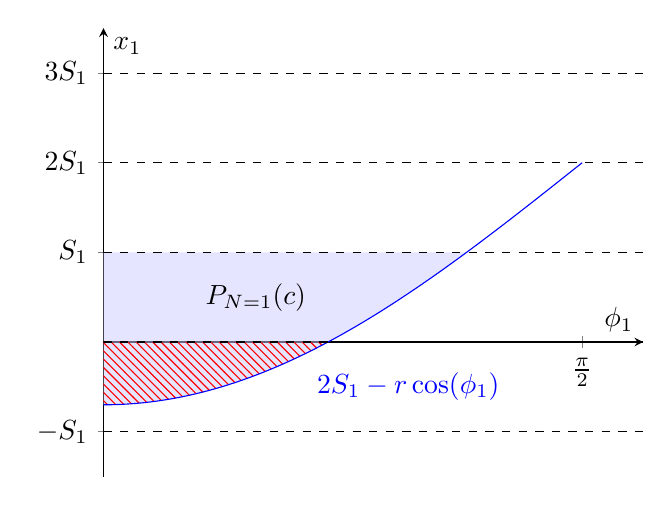
\begin{tikzpicture}
			\begin{axis}[
				axis lines=middle,
				xlabel={$\phi_1$},
				ylabel={$x_1$},
				xmin=0, xmax=pi/2+0.2, % Adjust the x-axis limits
				ymin=-1.5, ymax=3.5, % Adjust the y-axis limits
				xtick={0,pi/2}, % Adjust the x-axis tick positions
				ytick={-1,0,1,2,3}, % Adjust the y-axis tick positions
				xticklabels={0, $\frac{\pi}{2}$}, % Adjust the x-axis tick labels
				yticklabels={$-S_1$, 0, $S_1$, $2S_1$, $3S_1$}
			]

				% Parameters
				\def\S{1} % Replace with your desired value for S
				\def\r{2.7} % Replace with your desired value for r
				\def\c{2}
				\pgfmathsetmacro\endshaded{acos(\S*(\c-1)/\r)}

				% Plot the function
				\addplot[blue, domain=0:pi/2, samples=100, name path=curve] {\S*\c - \r*cos(deg(x))};
				% \addplot[red, domain=0:pi/2, samples=100, name path=Hcurve] {\S*(\c+1) - \r*cos(deg(x))};

				% Label the function
				\node[blue] at (axis cs:1,-.5) {$2S_1 - r\cos(\phi_1)$};
				\node at (axis cs:0.5,0.5) {$P_{N=1}(c)$};
				% \node[red] at (axis cs:1,2.5) {$3S_1 - r\cos(\phi_1)$};

				% Add dashed lines at -S, S, 2S, and 3S on the y-axis
				\draw[dashed] (axis cs:0,-\S) -- (axis cs:pi/2+0.2,-\S);
				\draw[dashed, name path = oline] (axis cs:0,0) -- (axis cs:pi/2+0.2,0);
				\draw[dashed, name path = Sline] (axis cs:0,\S) -- (axis cs:pi/2+0.2,\S);
				\draw[dashed] (axis cs:0,2*\S) -- (axis cs:pi/2+0.2,2*\S);
				\draw[dashed] (axis cs:0,3*\S) -- (axis cs:pi/2+0.2,3*\S);

				\addplot[blue!20, fill opacity=0.5] fill between[of=curve and Sline, soft clip={domain=0:1.191}];
				% \addplot[red!20, pattern=north west lines, pattern color=red] fill between[of=Hcurve and Sline, soft clip={domain=0:0.736}];
				\addplot[red!20, pattern=north west lines, pattern color=red] fill between[of=curve and oline, soft clip={domain=0:0.736}];

			\end{axis}
		\end{tikzpicture}
		\caption{The integral spanning the domain of the crossing condition can be found as a difference
		between two regions.}\label{fig:domains}
	\end{subfigure}
	\hspace{0.5cm}
	\begin{subfigure}{0.45\textwidth}
		\centering
		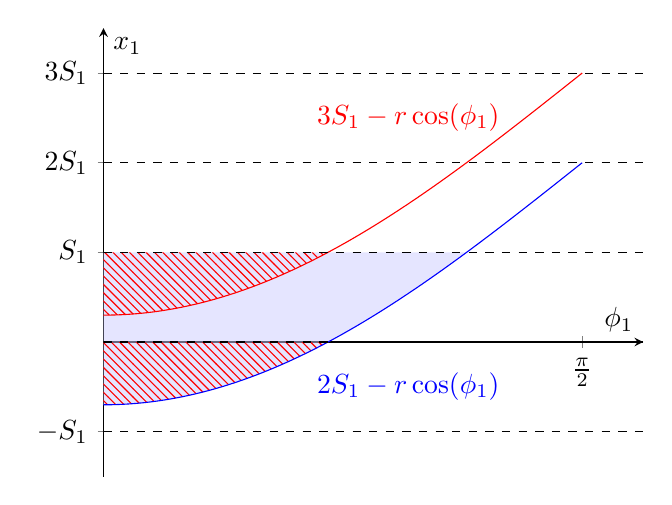
\begin{tikzpicture}
			\begin{axis}[
				axis lines=middle,
				xlabel={$\phi_1$},
				ylabel={$x_1$},
				xmin=0, xmax=pi/2+0.2, % Adjust the x-axis limits
				ymin=-1.5, ymax=3.5, % Adjust the y-axis limits
				xtick={0,pi/2}, % Adjust the x-axis tick positions
				ytick={-1,0,1,2,3}, % Adjust the y-axis tick positions
				xticklabels={0, $\frac{\pi}{2}$}, % Adjust the x-axis tick labels
				yticklabels={$-S_1$, 0, $S_1$, $2S_1$, $3S_1$}
			]

				% Parameters
				\def\S{1} % Replace with your desired value for S
				\def\r{2.7} % Replace with your desired value for r
				\def\c{2}
				\pgfmathsetmacro\endshaded{acos(\S*(\c-1)/\r)}

				% Plot the function
				\addplot[blue, domain=0:pi/2, samples=100, name path=curve] {\S*\c - \r*cos(deg(x))};
				\addplot[red, domain=0:pi/2, samples=100, name path=Hcurve] {\S*(\c+1) - \r*cos(deg(x))};

				% Label the function
				\node[blue] at (axis cs:1,-.5) {$2S_1 - r\cos(\phi_1)$};
				\node[red] at (axis cs:1,2.5) {$3S_1 - r\cos(\phi_1)$};

				% Add dashed lines at -S, S, 2S, and 3S on the y-axis
				\draw[dashed] (axis cs:0,-\S) -- (axis cs:pi/2+0.2,-\S);
				\draw[dashed, name path = oline] (axis cs:0,0) -- (axis cs:pi/2+0.2,0);
				\draw[dashed, name path = Sline] (axis cs:0,\S) -- (axis cs:pi/2+0.2,\S);
				\draw[dashed] (axis cs:0,2*\S) -- (axis cs:pi/2+0.2,2*\S);
				\draw[dashed] (axis cs:0,3*\S) -- (axis cs:pi/2+0.2,3*\S);

				\addplot[blue!20, fill opacity=0.5] fill between[of=curve and Sline, soft clip={domain=0:1.191}];
				\addplot[red!20, pattern=north west lines, pattern color=red] fill between[of=Hcurve and Sline, soft clip={domain=0:0.736}];
				\addplot[red!20, pattern=north west lines, pattern color=red] fill between[of=curve and oline, soft clip={domain=0:0.736}];

			\end{axis}
		\end{tikzpicture}
		\caption{Translational symmetry guarantees that the subtrahend is equivalent to the "short needle"
		probability of crossing an additional hyperplane.}\label{fig:long r int}
	\end{subfigure}
	\caption{}
\end{figure}

The integral $I_2$ is of the same form as the short needle case and can therefore be substituted with the
solution \ref{eq:n=1 final sol}. Using symmetry of the PDF in the $x_1$ direction, $I_3$ can be rewritten
with the limits of integration spanning $S_1(c+1)-r\cos\phi_1 < x_1 < S_1$. This is, again, exactly the problem of
the short needle case but with $c+1$ instead of $c$. This is visualized in Figure \ref{fig:long r int} As such, the result is
\begin{gather}
	P_{N=1}(c | r>S_1c) = A(c) - A(c+1) \\
	A(k) = \frac{r}{S_1} \left[\frac{(1-\gamma^2)^{\frac{D-1}{2}}}{\pi} \left(B\left(\frac{D}{2}, \frac{1}{2} \right) + \gamma^2 \sum_{i=1}^{\lfloor \frac{D-2}{2} \rfloor}\frac{B(\frac{D-2i}{2}, \frac{1}{2})}{(1-\gamma^2)^i}\right) - \gamma g(\gamma, D-2) \right] \\
	\gamma = \frac{S_1(k-1)}{r} \\
	g(n, m) = \begin{cases}
		\frac{2}{\pi}\arccos(n) & m\bmod 2 = 0 \\
		1-n & m \bmod 2 = 1
	\end{cases}
\end{gather}


\section{Probability of crossing $N\ge 1$}
When there is only a single set of parallel hyperplanes, there is only one way for a needle to make
$c$ intersections. The needle would have to go through $c$ hyperplanes in a single direction.
When we increase the number of orthogonal sets of hyperplanes then we must deal with the fact that
there are now many ways to cross $c$ hyperplanes due to the many combinations of directions available.

For instance, if $N=2$ and we want to know when $C=2$, then a valid number of crossings occurs if the
needle crosses 2 hyperplanes in $x_1$ and 0 in $x_2$, or 1 hyperplane in each direction, or 0 hyperplanes
in $x_1$ and 2 in $x_2$.

For simplicity, we begin with the assumption that $r<\min(S)$ to ensure that the needle can never cross
more than 1 hyperplane in any given direction.

\subsection{$N\ge 1, r<\min(S)$}
Let $P_{1\cap2\cap\hdots\cap h}(C=h|r,D,N,S)=P_{1\cap\hdots\cap h}$ be the probability that the
needle crosses exactly 1 hyperplane in every direction $x_1, x_2, \hdots, x_h$. Similarly,
let $P_{1\cup2\cup\hdots\cup h}(C\ge 1|r,D,N,S)=P_{1\cup\hdots\cup h}$ be the probability that
the needle crosses at least 1 hyperplane total in any direction $x_1, x_2, \hdots, x_h$. This probability
is equivalent to the probability that $P(C\ge 1|r,D,N,S)$ as crossing a hyperplane in any 
direction is sufficient to meet the condition $C\ge 1$. Using the inclusion-exclusion principle,
this probability can be written as the following sum.

\begin{equation}
	P(C\ge 1|r, D, N, S) = P_{1\cup2\cup\hdots\cup N} = \sum_{k=1}^N (-1)^{k+1}\left(\sum_{1\le i_1 < \hdots < i_k \le N}P_{i_1 \cap \hdots \cap i_k} \right)
\end{equation}

Similarly, for $C\ge c$, we can define the set of events $E_c^N$ which consists of each of the
$N \choose c$ hyperplane crossing combinations. For example, $E_2^3=\{(1,2), (1,3), (2,3)\}$.
If the needle crosses hyperplanes in all of the directions listed in any element of $E_c^N$,
then the crossing condition for the criteria $C \ge c$ has been met.

\begin{equation}
	P(C\ge c|r, D, N, S) = P_{(\cap E_c^N[1])\cup(\cap E_c^N[2])\cup\hdots\cup(\cap E_c^N[{N \choose c}])} = \sum_{k=1}^N (-1)^{k+1}\left(\sum_{1\le i_1 < \hdots < i_k \le N}P_{E_c^N[i_1] \cap \hdots \cap E_c^N[i_k]} \right)
\end{equation}

This expression requires an equation for the probability of having at least 1 crossing in
each direction listed. 

\begin{proposition}
	For any given set of hyperplane directions, $\emph{H}$, the probability that a needle would cross
	at least 1 hyperplane in each of the specified directions can be represented as follows.
	\begin{equation}
		P_{H_1 \cap \hdots \cap H_h} = \frac{r^h }{ \pi^{h/2} (\prod_{i=1}^h S_{H,i}) }\frac{\Gamma(\frac{D}{2})}{\Gamma(\frac{D+h}{2})}
	\end{equation}
\end{proposition}

\begin{proof}
	The set of hyperplane directions, $H$, with spacings $S_H$ is a subset of all the 
	hyperplanes that grid the space. Without loss of generalization, the axes can be relabeled to
	align $H_1$ with $x_1$, $H_2$ with $x_2$ and so on. All other hyperplanes that are not included
	in the set $H$ can be ignored as any intersections with them are irrelevant.

	The necessary conditions for crossings to occur in each direction specified in $H$ is as follows
	\begin{align}
		S_1 &\le x_1 + r\cos\phi_1\\
		S_2 &\le x_2 + r\sin\phi_1\cos\phi_2\\
		&\vdots \\
		S_{h-1} &\le x_{h-1} + r\sin\phi_1\sin\phi_2\hdots\sin\phi_{h-2}\cos\phi_{h-1}\\
		S_{h} &\le x_h + \begin{cases}
			r\sin\phi_1\hdots\sin\phi_{h-1}\cos\phi_{h} & h < D \\
			r\sin\phi_1\hdots\sin\phi_{h-2}\sin\phi_{h-1} & h = D
		\end{cases}
	\end{align}

	These conditions, along with the domain of $x_i \forall i\in {1,\hdots,h}$, define the bounds of the
	volume where the needle crosses a hyperplane in each direction $H$.
	
	\begin{align}
		S_1 \ge x_1 \ge m_1(\phi_1) &= \max\{0, S_1-r\cos\phi_1\}\\
		S_2 \ge x_2 \ge m_2(\phi_2) &= \max\{0, S_2-r\sin\phi_1\cos\phi_2\}\\
		&\vdots \\
		S_{h-1} \ge x_{h-1} \ge m_{h-1}(\phi_{h-1}) &= \max\{0, S_{h-1}-r\sin\phi_1\hdots\sin\phi_{h-2}\cos\phi_{h-1}\}\\
		S_h \ge x_h \ge m_{h}(\phi_{h}) &= \max\left\{0, S_h - \begin{cases}
			r\sin\phi_1\hdots\sin\phi_{h-1}\cos\phi_{h} & h < D\\
			r\sin\phi_1\hdots\sin\phi_{h-2}\sin\phi_{h-1} & h = D
		\end{cases} \right\}
	\end{align}
	Starting with \ref{eq:volume integral}, the crossing conditions above are encoded into
	the bounds of integration. As in the $N=1$ case, the order of integration is arbitrary
	so long as the limits of integration are not variable. Therefore the integrals with respect to the
	spatial dimensions greater than $h$ are reduced to a coefficient.

	\begin{align}
		P_{H_1\cap\hdots\cap H_h} &= \frac{2^{D-1}\Gamma(\frac{D}{2})}{\pi^{D/2}\prod_{i=1}^D S_i} \idotsint_V \prod_{j=1}^{D-1}\sin^{D-1-j}\phi_j dV \\
		&= \frac{2^{D-1}\Gamma(\frac{D}{2})}{\pi^{D/2}\prod_{i=1}^h S_i} \idotsint_{\phi}  \int_{m_h(\phi_h)}^{S_h} \hdots \int_{m_1(\phi_1)}^{S_1} \prod_{j=1}^{D-1}\sin^{D-1-j}\phi_j dx_1\hdots dx_h d\phi_1 \hdots d\phi_{D-1}
		% &= \frac{2^{D-1}\Gamma(\frac{D}{2})}{\pi^{D/2}\prod_{i=1}^h S_i} \prod_{k=h+1}^{D-1}\frac{B(\frac{D-k}{2}, \frac{1}{2})}{2} \idotsint_{\phi_1\hdots \phi_h x_1 \hdots x_h} \prod_{j=1}^{h}\sin^{D-1-j}\phi_j dx_1\hdots dx_h d\phi_1 \hdots d\phi_{h} \\
		% &= \frac{2^h}{\pi^{h/2}\prod_{i=1}^h S_i} \frac{\Gamma(\frac{D}{2})}{\Gamma(\frac{D-h}{2})} \idotsint_{\phi_1\hdots \phi_h x_1 \hdots x_h} \prod_{j=1}^{h}\sin^{D-1-j}\phi_j dx_1\hdots dx_h d\phi_1 \hdots d\phi_{h}
	\end{align}

		% &= \frac{2^{D-1}\Gamma(\frac{D}{2})}{\pi^{D\2}\prod_{i=1}^h S_i} \prod_{k=h+1}^{D-1}\frac{B(\frac{D-k}{2}, \frac{1}{2})}{2} \idotsint_{\phi_1\hdots \phi_h x_1 \hdots x_h}  \int_{m_h(\phi_h)}^{S_h} \hdots \int_{m_1(\phi_1)}^{S_1} \prod_{j=1}^{D-1}\sin^{D-1-j}\phi_j dx_1\hdots dx_h d\phi_1 \hdots d\phi_{D-1}

	Given that $r$ is less than every spacing $S_i$, every function $m_i(\phi_i)$ is guaranteed
	to be greater than zero. Every spatial integral will reduce to the polar representation of
	the corresponding $x_i$. This simplifies to the following.

	\begin{align}
		P_{H_1\cap\hdots\cap H_h} &= \frac{2^{D-1}\Gamma(\frac{D}{2})}{\pi^{D/2}\prod_{i=1}^h S_i} \idotsint_\phi r^h \left( \prod_{k=1}^{\min(D-1, h)} \cos\phi_k\sin^{h-k}\phi_k\right) \prod_{j=1}^{D-1}\sin^{D-1-j}\phi_j d\phi_1 \hdots d\phi_{D-1} \\
		&= \frac{2^{D-1}r^h\Gamma(\frac{D}{2})}{\pi^{D/2}\prod_{i=1}^h S_i} \idotsint_\phi \left( \prod_{k=1}^{\min(D-1, h)} \cos\phi_k\sin^{D+h-2k-1}\phi_k\right) \prod_{j=h+1}^{D-1}\sin^{D-1-j}\phi_j d\phi_1 \hdots d\phi_{D-1}
	\end{align}

	The product from $k=1$ to $\min(D-1,h)$ can be reduced by using u-substitution where 
	$u=\sin\phi_k$. Assuming that $h\le D-1$, this results as follows

	\begin{align}
		P_{H_1\cap\hdots\cap H_h} &= \frac{2^{D-1}r^h\Gamma(\frac{D}{2})}{\pi^{D/2}\prod_{i=1}^h S_i} \idotsint_0^{\pi/2} \frac{1}{(D+h-2)(D+h-4)\hdots(D-h)} \prod_{j=h+1}^{D-1}\sin^{D-1-j}\phi_j d\phi_{h+1} \hdots d\phi_{D-1} \\
		&= \frac{2^{D-1}r^h\Gamma(\frac{D}{2})}{\pi^{D/2}\prod_{i=1}^h S_i} \frac{(D-h-2)!!}{(D+h-2)!!} \idotsint_0^{\pi/2} \prod_{j=h+1}^{D-1}\sin^{D-1-j}\phi_j d\phi_{h+1} \hdots d\phi_{D-1} \\
		&= \frac{2^{D-1}r^h\Gamma(\frac{D}{2})}{\pi^{D/2}\prod_{i=1}^h S_i} \frac{\Gamma(\frac{D-h}{2})}{2^h \Gamma(\frac{D+h}{2})} \prod_{j=h+1}^{D-1}\frac{B(\frac{D-j}{2}, \frac{1}{2})}{2} \\
		&= \frac{r^{h}}{\pi^{h/2}\prod_{i=1}^h S_i} \frac{\Gamma(\frac{D}{2})}{\Gamma(\frac{D+h}{2})} \\
	\end{align}

	If $h$ is greater than $D-1$ (ie. $h=D$), the result remains the same.
	\begin{align}
		P_{H_1\cap\hdots\cap H_h} &= \frac{2^Dr^{D+h-1}}{A_{D-1}\prod_{i=1}^h S_i}  \frac{1}{(D+h-2)(D+h-4)\hdots(4)(2)}  \\
		&= \frac{2^Dr^{h} \Gamma(\frac{D}{2})}{2 \pi^{D/2} \prod_{i=1}^h S_i} \frac{1}{(D+h-2)!!} \\
		&= \frac{2^Dr^{h} \Gamma(\frac{D}{2})}{2 \pi^{D/2} \prod_{i=1}^h S_i} \frac{1}{2^{(D+h-2)/2} \Gamma(\frac{D+h}{2})} \\
		&= \frac{r^{h}}{\pi^{h/2} \prod_{i=1}^h S_i} \frac{\Gamma(\frac{D}{2})}{\Gamma(\frac{D+h}{2})} \\
	\end{align}


\end{proof}

\section{Numeric Simulation of Crossing and Other Conditions when $N=1$} \label{s:n=1 numeric}
To summarize, the probability that a randomly placed line segment will cross at least $c$
hyperplanes given that there is 1 set of parallel hyperplanes with spacing $S_1$ is as follows

\begin{gather*}
	P(C\ge c | r, D, N=1, S) = \begin{cases}
		0 & r < S(c-1) \\ 
		A(c)  & S_1 (c-1) < r < S_1 c \\
		A(c) - A(c+1) & r > S_1c		
	\end{cases} \\
	A(k) = \frac{r}{S_1} \left[\frac{(1-\gamma^2)^{\frac{D-1}{2}}}{\pi} \left(B\left(\frac{D}{2}, \frac{1}{2} \right) + \gamma^2 \sum_{i=1}^{\lfloor \frac{D-2}{2} \rfloor}\frac{B(\frac{D-2i}{2}, \frac{1}{2})}{(1-\gamma^2)^i}\right) - \gamma g(\gamma, D-2) \right] \\
	\gamma = \frac{S_1(k-1)}{r},\ g(n, m) = \begin{cases}
		\frac{2}{\pi}\arccos(n) & m\bmod 2 = 0 \\
		1-n & m \bmod 2 = 1
	\end{cases}
\end{gather*}

To compare this against numeric simulation, many samples of a randomly placed needle must be generated.
The initial point of the needle, $P_0$, is simulated using a uniformly distributed random variable in 
the domain $(\vec 0, S)$ and has coordinates $\vec x \in \mathbb{R}^D$. For the other point of the needle, $P_1$, samples 
with uniform spherical distribution must be generated for higher dimensional space. We use the method
proposed by Marsaglia \todo{ref} of normalizing a rotationally symmetric distribution 
(such as a D-dimensional gaussian variable) and label these coordinates as $\vec y \in \mathbb{R}^D$. For a needle of
length $r$, the point $P_1$ is then at the point $\vec x + r \vec y$.

The number of hyperplanes crossed by the needle in each coordinate is then of the following form.
\begin{equation}
	c = \sum_{n=1}^{N} \left|\left\lfloor \frac{x_n+r y_n}{S_n} \right\rfloor\right|
\end{equation}

The expected value of the probability can then be approximated by simulating many needles, checking
how many have satisfied the number of crossings, and dividing by the total number of simulations.
The above procedure was simulated for 100,000 randomly generated needles for each permutation of parameters
listed below\footnote{For a total of 363.6 million needles} and results shown in Figure \ref{fig:numeric sim N1}. The probabilities were calculated for
$c\in\{1,2,3,4\}$, needle length $r\in(0, 10]$, dimensions $D\in[2, 10]$, a single hyperplane with
spacing $S_1=1$.

\begin{figure}
	\centerline{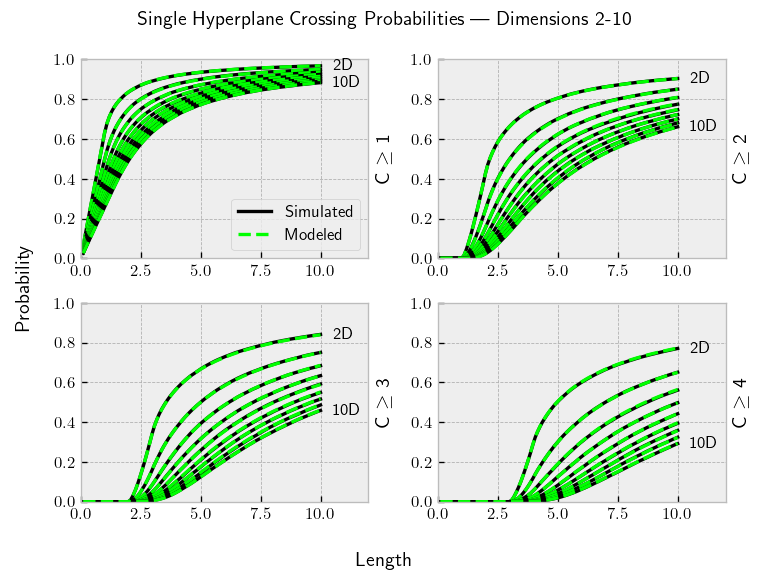
\includegraphics[width=5in]{numeric_sim_N1.png}}
	\caption{Comparison of numerically simulated and modeled probabilities for a variety of parameters.
	100,000 needles were simulated for every parameter permutation.}
	\label{fig:numeric sim N1}
\end{figure}

Similarly, the count of intersections can be compared to an exact number of crossings as well. The modeled
probability can be calculated as follows.

\begin{gather}
	P(C=c|r, D, N=1, S) = P(C\ge c|r, D, N=1, S) - P(C\ge c+1|r, D, N=1, S)
\end{gather}

\begin{figure}
	\centerline{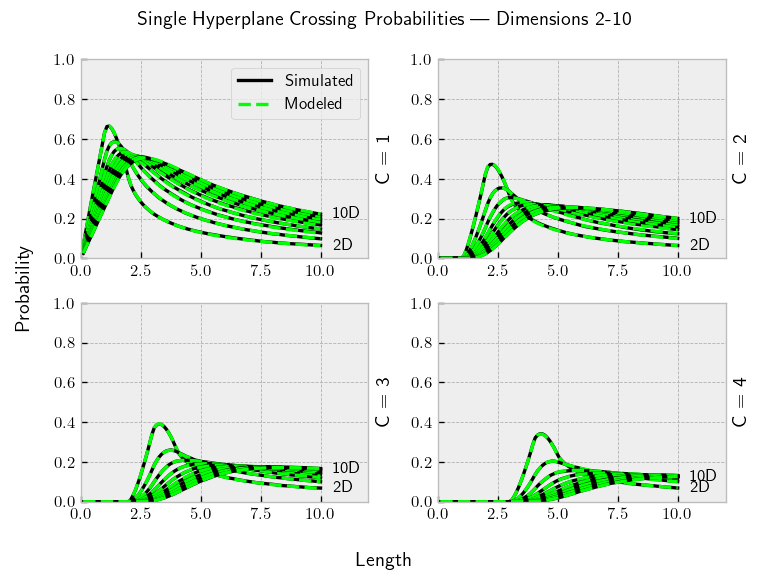
\includegraphics[width=5in]{numeric_sim_N1_e.png}}
	\caption{Numeric and modeled probability for exactly $c$ needle crossings.}
	\label{fig:numeric sim N1 e}
\end{figure}

The simulated and modeled probabilities can be found in Figure \ref{fig:numeric sim N1 e}. In the exact
crossing condition, there is a needle length that maximizes the probability that a certain number of crossings
occur. This can be calculated by taking the derivative of the expression for $P(C=c)$ with respect to $r$
and setting it equal to zero.

\begin{gather}
	\frac{d}{dr}\gamma(k) = -\frac{S_1(k-1)}{r^2} \\
	\frac{d}{dr}A(k) = \frac{A(k)}{r}+\frac{r}{S_1}\left( \frac{}{} \right) \\
	\frac{d}{dr}P(C=c|r,D,N=1,S) = 0 = \begin{cases}
		0 & r<S_1(c-1) \\
		\frac{d}{dr}A(c) - 0 & S_1(c-1) < r < S_1 \\
		\frac{d}{dr}A(c) - \frac{d}{dr}(2A(c+1)) & S_1c<r<S_1(c+1) \\
		\frac{d}{dr}A(c) - \frac{d}{dr}(2A(c+1)) + \frac{d}{dr}A(c+2) & r>S_1(c+1)
	\end{cases}
\end{gather}

% template stuff
\section{Examples of citations, figures, tables, references}
\label{sec:others}

\subsection{Citations}
Citations use \verb+natbib+. The documentation may be found at
\begin{center}
	\url{http://mirrors.ctan.org/macros/latex/contrib/natbib/natnotes.pdf}
\end{center}

Here is an example usage of the two main commands (\verb+citet+ and \verb+citep+): Some people thought a
thing \citep{kour2014real, hadash2018estimate} but other people thought something else \citep{kour2014fast}. 
Many people have speculated that if we knew exactly why \citet{kour2014fast} thought this\dots


The documentation for \verb+booktabs+ (`Publication quality tables in LaTeX') is available from:
\begin{center}
	\url{https://www.ctan.org/pkg/booktabs}
\end{center}

\bibliographystyle{unsrtnat}
\bibliography{references}  %%% Uncomment this line and comment out the ``thebibliography'' section below to use the external .bib file (using bibtex) .


%%% Uncomment this section and comment out the \bibliography{references} line above to use inline references.
% \begin{thebibliography}{1}

% 	\bibitem{kour2014real}
% 	George Kour and Raid Saabne.
% 	\newblock Real-time segmentation of on-line handwritten arabic script.
% 	\newblock In {\em Frontiers in Handwriting Recognition (ICFHR), 2014 14th
% 			International Conference on}, pages 417--422. IEEE, 2014.

% 	\bibitem{kour2014fast}
% 	George Kour and Raid Saabne.
% 	\newblock Fast classification of handwritten on-line arabic characters.
% 	\newblock In {\em Soft Computing and Pattern Recognition (SoCPaR), 2014 6th
% 			International Conference of}, pages 312--318. IEEE, 2014.

% 	\bibitem{hadash2018estimate}
% 	Guy Hadash, Einat Kermany, Boaz Carmeli, Ofer Lavi, George Kour, and Alon
% 	Jacovi.
% 	\newblock Estimate and replace: A novel approach to integrating deep neural
% 	networks with existing applications.
% 	\newblock {\em arXiv preprint arXiv:1804.09028}, 2018.

% \end{thebibliography}


\end{document}
